% =========================================================
% CHƯƠNG III: PHÂN TÍCH VÀ THIẾT KẾ HỆ THỐNG
% =========================================================

\chapter{Phân tích và thiết kế hệ thống}
\label{ch:thietke}

\begin{infobox}
\textbf{Mục tiêu chương:} 
Chương này thực hiện phân tích bài toán và các yêu cầu hệ thống, thiết kế kiến trúc phân tầng tổng thể trên nền tảng Cloud phân tán (Vercel, Render, TiDB Cloud), chuẩn hóa lược đồ cơ sở dữ liệu quan hệ gồm 6 bảng dữ liệu cốt lõi; đồng thời đóng vai trò như một tài liệu đặc tả kỹ thuật chi tiết (Software Requirements Specification -- SRS) mô tả toàn bộ 10 ca sử dụng cùng các biểu đồ luồng hoạt động và máy trạng thái của hệ sinh thái GiftAI.
\end{infobox}

% =====================================================================
% PHẦN I: PHÂN TÍCH VÀ THIẾT KẾ HỆ THỐNG
% =====================================================================

\section{Phân tích bài toán và yêu cầu hệ thống}

\subsection{Bối cảnh bài toán và phát biểu bài toán}
Quá trình lựa chọn một món quà tặng là sự kết hợp phức tạp giữa các yếu tố định tính (cảm xúc, mối quan hệ, sự tinh tế) và định lượng (ngân sách, độ tuổi, tính hữu dụng). Hệ thống GiftAI giải quyết bài toán ánh xạ từ nhu cầu tự nhiên của người tặng $\mathcal{U}_{\mathrm{input}}$ sang một danh mục sản phẩm tối ưu $\mathcal{R}^*$ từ kho hàng thương mại điện tử thực tế:
\begin{equation}
f: \mathcal{U}_{\mathrm{input}} \xrightarrow{\quad \text{Intent Parsing} \quad} \mathcal{K}_{\mathrm{search}} \xrightarrow{\quad \text{Database Query / Web Scraping} \quad} \mathcal{P}_{\mathrm{raw}} \xrightarrow{\quad \text{LLM Re-ranking} \quad} \mathcal{R}^*.
\end{equation}

\subsection{Yêu cầu chức năng (Functional Requirements)}
\begin{itemize}[leftmargin=1.2cm, itemsep=2pt]
    \item \textbf{Phân tích nhu cầu tự nhiên:} Tiếp nhận văn bản tự do tiếng Việt kết hợp các bộ lọc thuộc tính định lượng (đối tượng, dịp lễ, độ tuổi, khoảng giá).
    \item \textbf{Truy xuất và Re-ranking thông minh:} Truy vấn kho $1.400+$ sản phẩm quà tặng từ TiDB Cloud (kết hợp cào bù thời gian thực từ Shopee/Lazada) và sử dụng Gemini 3.8 Flash để loại bỏ hàng phụ kiện lệch tông, chọn lọc danh mục quà hoàn hảo nhất kèm lý giải tâm lý thuyết phục.
    \item \textbf{Sinh thiệp chúc mừng tự động (AI Greeting Card):} Sáng tác thông điệp chúc mừng theo nhiều phong cách biểu cảm, hỗ trợ xem trước và tương tác mở thiệp pháo hoa.
    \item \textbf{Hộp quà kỷ niệm ảo (Virtual Memory Box):} Lưu trữ tâm thư, gắn quà tặng thực tế, đếm xuôi ngày bên nhau hoặc đếm ngược sự kiện, chia sẻ qua mã \texttt{share\_code} độc bản dạng \texttt{MEM-XXXXXX}.
    \item \textbf{Cá nhân hóa người dùng:} Lưu danh sách quà yêu thích thả tim (\texttt{user\_favorites}) và lịch sử tìm kiếm có snapshot sản phẩm (\texttt{search\_history}).
    \item \textbf{Quản trị và đo lường (Admin Analytics):} Theo dõi số lượt nhấp chuột vào sản phẩm, tỷ lệ CTR và trạng thái hoạt động của các khóa API trên trang Dashboard.
\end{itemize}

\subsection{Yêu cầu phi chức năng (Non-functional Requirements)}
\begin{itemize}[leftmargin=1.2cm, itemsep=2pt]
    \item \textbf{Thời gian đáp ứng (Performance):} Phản hồi tức thì dưới $10\text{ ms}$ đối với các yêu cầu đã có trong RAM Cache; dưới $2.5\text{ giây}$ cho toàn bộ tiến trình truy vấn kho TiDB Cloud và tái xếp hạng qua LLM.
    \item \textbf{Tính sẵn sàng và chịu lỗi (Fault Tolerance):} Hệ thống duy trì hoạt động 24/7; tự động xoay vòng đa khóa API khi gặp lỗi giới hạn hạn ngạch (HTTP 429) và chuyển mạch dự phòng sang Groq hoặc OpenAI khi Gemini quá tải.
    \item \textbf{Bảo mật dữ liệu (Security):} Mật khẩu người dùng được băm an toàn qua thuật toán \texttt{bcrypt} (10 salt rounds); phiên làm việc được bảo vệ bằng JSON Web Token (JWT); đường truyền kết nối CSDL TiDB Cloud bắt buộc mã hóa qua SSL/TLSv1.2.
    \item \textbf{Tính tương thích (Compatibility):} Giao diện Web thích ứng linh hoạt (Responsive) trên mọi kích thước màn hình, triển khai trên Vercel và chạy mượt mà trên ứng dụng Android Native WebView container.
\end{itemize}

% ---------------------------------------------------------------------
\section{Thiết kế kiến trúc hệ thống (System Architecture Design)}

\subsection{Mô hình kiến trúc phân tầng trên môi trường Cloud}
Hệ thống GiftAI được thiết kế theo mô hình kiến trúc phân tầng (\textit{Multi-tier Cloud Architecture}) phân tách độc lập trách nhiệm giữa các khối như thể hiện tại Hình~\ref{fig:sys_struct}:

\begin{figure}[htbp]
\centering
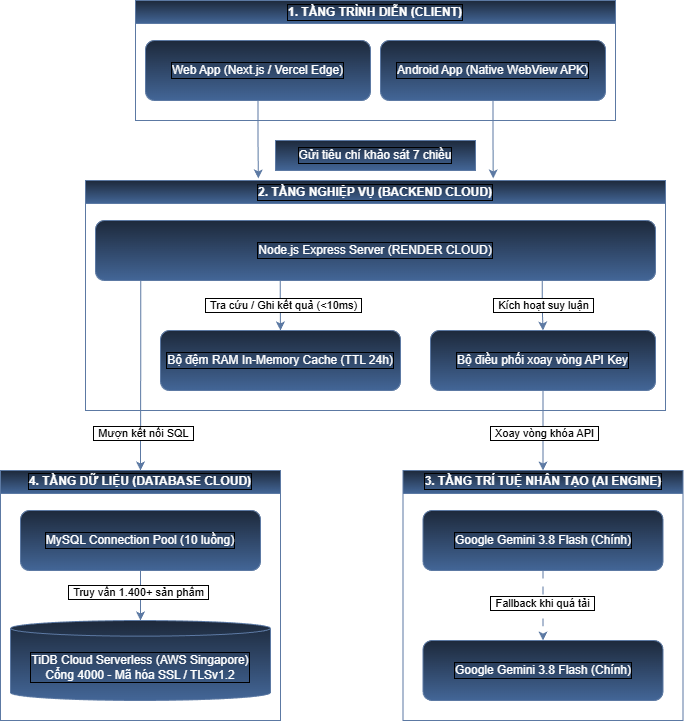
\includegraphics[width=0.7\textwidth]{chapters/diagram/Struct.drawio.png}
\caption{Kiến trúc phân tầng tổng thể của hệ thống GiftAI.}
\label{fig:sys_struct}
\end{figure}

Sơ đồ trên biểu diễn 4 tầng kiến trúc phân tách độc lập của hệ thống GiftAI trên môi trường đám mây thực tế. Tầng Giao diện (Presentation Tier) gồm ứng dụng Web SPA xây dựng bằng React 19/TypeScript triển khai trên mạng lưới toàn cầu Vercel và ứng dụng di động Android Native WebView container. Tầng Điều phối ứng dụng (Application Tier) chạy trên nền tảng Render, sử dụng Node.js Express cung cấp các RESTful API, quản lý bộ đệm RAM Cache và duy trì nhóm 10 kết nối thường trực (\textit{Connection Pool}) tới CSDL. Tầng Trí tuệ Nhân tạo \& Cào dữ liệu (AI \& Crawler Tier) tích hợp Google Gemini 3.8 Flash làm mô hình suy luận chính, Groq LPU làm bộ chuyển mạch dự phòng siêu tốc, kết hợp trình duyệt ngầm Selenium thu thập sản phẩm từ Shopee/Lazada. Cuối cùng, Tầng Cơ sở dữ liệu (Data Tier) sử dụng TiDB Cloud Serverless tại cụm máy chủ AWS Singapore, kết nối bảo mật qua SSL/TLSv1.2 ở cổng 4000. Việc phân tách này giúp từng tầng có thể mở rộng độc lập, tối ưu hóa thời gian phản hồi chỉ còn 1.5 đến 2.5 giây đối với mỗi phiên tư vấn quà tặng.

\subsection{Nguyên tắc phân chia trách nhiệm}

\begin{table}[htbp]
\centering
\caption{Phân chia trách nhiệm giữa các thành phần trong hệ thống GiftAI.}
\label{tab:component_responsibility}
\small
\renewcommand{\arraystretch}{1.25}
\begin{tabularx}{\textwidth}{|p{3.8cm}|X|}
\hline
\rowcolor{PrimaryBlue}
\textcolor{white}{\textbf{Thành phần}} & \textcolor{white}{\textbf{Trách nhiệm đảm nhiệm}} \\
\hline
Web SPA (Vercel) / Android Client & Tiếp nhận thông tin tìm quà; hiển thị danh sách đề xuất; tương tác tạo thiệp và mở hộp quà. \\
\hline
Express Backend Server (Render) & Xác thực dữ liệu; điều phối luồng nghiệp vụ; quản lý phiên JWT; duy trì Connection Pool 10 luồng và kiểm soát bộ đệm RAM Cache. \\
\hline
Module AI Manager & Bóc tách ý định người dùng; xoay vòng khóa API theo vòng tròn modulo; chuyển đổi dự phòng mô hình (Gemini sang Groq/OpenAI); tái xếp hạng sản phẩm. \\
\hline
Web Scraper Workers & Tự động hóa trình duyệt Chrome không đầu thu thập sản phẩm từ sàn TMĐT (Shopee, Lazada) khi cần cập nhật kho. \\
\hline
TiDB Cloud Database & Lưu trữ dữ liệu cấu hình, kho 1.400+ sản phẩm, tài khoản người dùng, danh mục yêu thích, hộp quà số và lịch sử tìm kiếm. \\
\hline
\end{tabularx}
\end{table}

Bảng trên phân định rõ ranh giới trách nhiệm của từng thành phần phần mềm trong toàn bộ hệ thống. Mỗi thành phần hoạt động theo mô hình phi tập trung hóa và giao tiếp với nhau qua các giao thức mạng chuẩn như HTTP RESTful và giao thức MySQL có mã hóa TLS. Thiết kế này đem lại tính mô-đun hóa cao (\textit{High Modularity}), giúp đội ngũ phát triển dễ dàng nâng cấp từng thành phần (chẳng hạn thay đổi mô hình AI từ Gemini 3.8 Flash sang một mô hình mới hơn) mà không làm ảnh hưởng tới giao diện người dùng hay cấu trúc dữ liệu lưu trữ phía dưới.

% ---------------------------------------------------------------------
\section{Thiết kế cơ sở dữ liệu quan hệ phân tán (TiDB Cloud Schema)}

Cơ sở dữ liệu của GiftAI được triển khai trên nền tảng TiDB Cloud (AWS Singapore, Port 4000, mã hóa SSL/TLSv1.2), đạt chuẩn chuẩn hóa 3NF (\textit{Third Normal Form}) kết hợp các trường kiểu \texttt{JSON} linh hoạt. Toàn bộ 6 bảng dữ liệu cốt lõi được đặc tả chi tiết từ Bảng~\ref{tab:db_scraped_products} đến Bảng~\ref{tab:db_memory}.

% BẢNG 1: SCRAPED_PRODUCTS
\begin{table}[htbp]
\centering
\caption{Đặc tả chi tiết bảng kho sản phẩm và cache quà tặng (\texttt{scraped\_products}).}
\label{tab:db_scraped_products}
\small
\renewcommand{\arraystretch}{1.25}
\begin{tabularx}{\textwidth}{|p{3.0cm}|p{2.6cm}|p{2.8cm}|X|}
\hline
\rowcolor{PrimaryBlue}
\textcolor{white}{\textbf{Tên trường}} &
\textcolor{white}{\textbf{Kiểu dữ liệu}} &
\textcolor{white}{\textbf{Ràng buộc}} &
\textcolor{white}{\textbf{Mô tả ý nghĩa nghiệp vụ}} \\
\hline
\texttt{id} & INT & PK, Auto & Khóa chính định danh duy nhất của sản phẩm. \\
\hline
\texttt{product\_key} & VARCHAR(500) & Unique, Not Null & Khóa định danh duy nhất (URL hash) chống trùng lặp khi cào. \\
\hline
\texttt{platform} & VARCHAR(100) & Not Null & Sàn TMĐT nguồn (lazada, shopee, tiki,...). \\
\hline
\texttt{name} & VARCHAR(1000) & Not Null & Tên thương mại đầy đủ của món quà. \\
\hline
\texttt{price} & DECIMAL(15,2) & Nullable & Giá bán thực tế của sản phẩm (VNĐ). \\
\hline
\texttt{currency} & VARCHAR(20) & Default 'VND' & Đơn vị tiền tệ giao dịch. \\
\hline
\texttt{image} & TEXT & Nullable & Đường dẫn hình ảnh đại diện của sản phẩm. \\
\hline
\texttt{url} & TEXT & Nullable & Liên kết dẫn trực tiếp tới gian hàng bán sản phẩm. \\
\hline
\texttt{category} & VARCHAR(255) & Default 'Product' & Ngành hàng (Công nghệ, Thời trang, Quà lưu niệm,...). \\
\hline
\texttt{condition\_name} & VARCHAR(255) & Default 'New' & Tình trạng sản phẩm (Mới 100\%, Nguyên hộp). \\
\hline
\texttt{location} & VARCHAR(255) & Default 'Vietnam' & Khu vực địa lý của gian hàng người bán. \\
\hline
\texttt{search\_keyword} & VARCHAR(500) & Not Null, Index & Từ khóa danh mục quà tặng phục vụ truy vấn cache nhanh. \\
\hline
\texttt{score} & DECIMAL(5,2) & Default 0 & Điểm đánh giá độ phù hợp mặc định. \\
\hline
\texttt{reason} & TEXT & Nullable & Lời giải thích lý do gợi ý mẫu sinh sẵn. \\
\hline
\texttt{created\_at} & TIMESTAMP & Default NOW() & Thời điểm bản ghi được thu thập và lưu trữ. \\
\hline
\texttt{updated\_at} & TIMESTAMP & On Update NOW(), Index & Thời điểm cập nhật biến động giá hoặc tồn kho. \\
\hline
\end{tabularx}
\end{table}

Bảng \texttt{scraped\_products} gồm 16 cột dữ liệu, đóng vai trò là danh mục hàng hóa trung tâm lưu trữ hơn $1.400+$ sản phẩm quà tặng được chọn lọc từ các sàn thương mại điện tử lớn và tập dữ liệu khởi tạo (\textit{Seed data}). Việc thiết lập ràng buộc \texttt{UNIQUE} trên cột \texttt{product\_key} cho phép hệ thống sử dụng cú pháp \texttt{INSERT ... ON DUPLICATE KEY UPDATE}, nhờ đó các tiến trình cào dữ liệu chạy nền có thể tự động cập nhật biến động giá hoặc đường dẫn ảnh mà không bao giờ làm trùng lặp dữ liệu. Cột \texttt{search\_keyword} và \texttt{updated\_at} được đánh chỉ mục giúp Backend truy xuất danh mục quà tặng phù hợp với từ khóa người dùng chỉ trong vòng $5 - 10\text{ ms}$, giải quyết triệt để nút thắt cổ chai về độ trễ khi tìm kiếm quà tặng trực tuyến.

% BẢNG 2: USERS
\begin{table}[htbp]
\centering
\caption{Đặc tả chi tiết bảng quản lý tài khoản người dùng (\texttt{users}).}
\label{tab:db_users}
\small
\renewcommand{\arraystretch}{1.25}
\begin{tabularx}{\textwidth}{|p{3.0cm}|p{2.6cm}|p{2.8cm}|X|}
\hline
\rowcolor{PrimaryBlue}
\textcolor{white}{\textbf{Tên trường}} &
\textcolor{white}{\textbf{Kiểu dữ liệu}} &
\textcolor{white}{\textbf{Ràng buộc}} &
\textcolor{white}{\textbf{Mô tả ý nghĩa nghiệp vụ}} \\
\hline
\texttt{id} & INT & PK, Auto & Khóa chính định danh tài khoản người dùng. \\
\hline
\texttt{email} & VARCHAR(255) & Unique, Not Null, Index & Địa chỉ email dùng để xác thực và đăng nhập. \\
\hline
\texttt{password\_hash} & VARCHAR(255) & Not Null & Chuỗi mật khẩu băm bảo mật bằng thuật toán bcrypt. \\
\hline
\texttt{full\_name} & VARCHAR(255) & Not Null & Họ và tên hiển thị của người dùng. \\
\hline
\texttt{role} & ENUM('user','admin') & Default 'user', Index & Phân quyền truy cập (user: người dùng, admin: quản trị). \\
\hline
\texttt{avatar\_url} & VARCHAR(500) & Nullable & Liên kết ảnh đại diện cá nhân của người dùng. \\
\hline
\texttt{created\_at} & TIMESTAMP & Default NOW() & Thời điểm người dùng đăng ký tài khoản. \\
\hline
\texttt{updated\_at} & TIMESTAMP & On Update NOW() & Thời điểm cập nhật thông tin hồ sơ cá nhân. \\
\hline
\end{tabularx}
\end{table}

Bảng \texttt{users} gồm 8 trường dữ liệu chịu trách nhiệm quản lý định danh người dùng và kiểm soát phân quyền trong toàn bộ hệ thống. Mật khẩu không bao giờ được lưu dưới dạng chuỗi thuần mà bắt buộc phải băm một chiều qua thuật toán \texttt{bcryptjs} với chi phí băm 10 vòng muối (\textit{Salt rounds}), đảm bảo an toàn tuyệt đối trước các cuộc tấn công tra cứu bảng cầu vồng. Trường \texttt{role} định nghĩa hai cấp độ truy cập: người dùng thông thường (\texttt{'user'}) và quản trị viên (\texttt{'admin'}). Việc đánh chỉ mục trên cột \texttt{email} giúp quá trình xác thực đăng nhập và giải mã chữ ký số JSON Web Token (JWT) diễn ra trong thời gian dưới $5\text{ ms}$.

% BẢNG 3: SEARCH_HISTORY
\begin{table}[htbp]
\centering
\caption{Đặc tả chi tiết bảng lịch sử tìm kiếm và snapshot AI (\texttt{search\_history}).}
\label{tab:db_history}
\small
\renewcommand{\arraystretch}{1.25}
\begin{tabularx}{\textwidth}{|p{3.0cm}|p{2.6cm}|p{2.8cm}|X|}
\hline
\rowcolor{PrimaryBlue}
\textcolor{white}{\textbf{Tên trường}} &
\textcolor{white}{\textbf{Kiểu dữ liệu}} &
\textcolor{white}{\textbf{Ràng buộc}} &
\textcolor{white}{\textbf{Mô tả ý nghĩa nghiệp vụ}} \\
\hline
\texttt{id} & INT & PK, Auto & Khóa chính của phiên tư vấn tìm kiếm. \\
\hline
\texttt{user\_id} & INT & FK, Nullable, Index & Khóa ngoại liên kết tới bảng \texttt{users} (NULL nếu vãng lai). \\
\hline
\texttt{query\_text} & TEXT & Nullable & Chuỗi văn bản mô tả tự do của người dùng. \\
\hline
\texttt{relationship} & VARCHAR(100) & Nullable, Index & Đối tượng nhận quà (Người yêu, Bố mẹ, Bạn bè, Sếp,...). \\
\hline
\texttt{gender} & VARCHAR(50) & Nullable & Giới tính của người nhận quà (Nam, Nữ, Khác). \\
\hline
\texttt{age\_range} & VARCHAR(50) & Nullable & Khung độ tuổi người nhận (Dưới 18, 18-24, 25-34,...). \\
\hline
\texttt{occasion} & VARCHAR(100) & Nullable, Index & Dịp tặng quà (Sinh nhật, Valentine, Tân gia, 20/10,...). \\
\hline
\texttt{budget} & VARCHAR(100) & Nullable & Khung ngân sách dự kiến (Dưới 200k, 200k-500k,...). \\
\hline
\texttt{interests} & JSON & Nullable & Mảng JSON lưu trữ danh sách sở thích và tính cách. \\
\hline
\texttt{ai\_summary} & TEXT & Nullable & Bản tóm tắt phân tích tâm lý người nhận từ Gemini. \\
\hline
\texttt{ai\_keywords} & JSON & Nullable & Mảng các từ khóa tìm kiếm cốt lõi do AI trích xuất. \\
\hline
\texttt{ai\_items} & JSON & Nullable & Mảng các ý tưởng quà tặng dạng văn bản do AI đề xuất. \\
\hline
\texttt{products\_snapshot} & JSON & Nullable & Snapshot JSON lưu nguyên trạng danh sách quà tại thời điểm tìm. \\
\hline
\texttt{total\_products} & INT & Default 0 & Số lượng sản phẩm thỏa mãn được hiển thị. \\
\hline
\texttt{ip\_address} & VARCHAR(100) & Nullable & Địa chỉ IP của máy khách thực hiện truy vấn. \\
\hline
\texttt{created\_at} & TIMESTAMP & Default NOW(), Index & Thời điểm phiên tìm kiếm được thực thi. \\
\hline
\end{tabularx}
\end{table}

Bảng \texttt{search\_history} gồm 16 trường dữ liệu ghi nhận đầy đủ mọi phiên tư vấn quà tặng của cả người dùng vãng lai (\texttt{user\_id = NULL}) và thành viên đã đăng nhập. Cột \texttt{products\_snapshot} đóng vai trò như một bản chụp nhanh nguyên trạng (\textit{Snapshot}): lưu trữ toàn bộ thông tin giá, ảnh, liên kết của danh sách quà tặng tại thời điểm tư vấn dưới định dạng JSON nguyên bản của TiDB Cloud. Thiết kế này giúp người dùng khi mở lại lịch sử có thể xem ngay kết quả cũ mà không cần máy chủ phải thực hiện các phép kết (\textit{JOIN}) phức tạp, đồng thời bảo toàn mức giá thực tế tại thời điểm đề xuất kể cả khi giá sản phẩm trên sàn TMĐT có biến động sau này.

% BẢNG 4: PRODUCT_RECOMMENDATION_STATS
\begin{table}[htbp]
\centering
\caption{Đặc tả chi tiết bảng đo lường tương tác quà tặng (\texttt{product\_recommendation\_stats}).}
\label{tab:db_stats}
\small
\renewcommand{\arraystretch}{1.25}
\begin{tabularx}{\textwidth}{|p{3.0cm}|p{2.6cm}|p{2.8cm}|X|}
\hline
\rowcolor{PrimaryBlue}
\textcolor{white}{\textbf{Tên trường}} &
\textcolor{white}{\textbf{Kiểu dữ liệu}} &
\textcolor{white}{\textbf{Ràng buộc}} &
\textcolor{white}{\textbf{Mô tả ý nghĩa nghiệp vụ}} \\
\hline
\texttt{id} & INT & PK, Auto & Khóa chính của bản ghi thống kê. \\
\hline
\texttt{search\_history\_id} & INT & FK, Nullable, Index & Khóa ngoại liên kết tới phiên trong \texttt{search\_history}. \\
\hline
\texttt{product\_name} & VARCHAR(500) & Not Null, Index(100) & Tên món quà được AI đề xuất cho người dùng. \\
\hline
\texttt{product\_price} & DECIMAL(15,2) & Nullable & Giá bán của sản phẩm tại thời điểm gợi ý. \\
\hline
\texttt{product\_image} & TEXT & Nullable & Đường dẫn hình ảnh minh họa của sản phẩm. \\
\hline
\texttt{product\_url} & TEXT & Nullable & Đường dẫn tiếp thị chuyển hướng mua hàng. \\
\hline
\texttt{platform} & VARCHAR(100) & Default 'lazada', Index & Nền tảng bán hàng nguồn. \\
\hline
\texttt{score} & DECIMAL(5,2) & Default 0 & Điểm tương hợp do AI thẩm định. \\
\hline
\texttt{clicks} & INT & Default 0 & Số lượt người dùng nhấn vào nút xem chi tiết / mua quà. \\
\hline
\texttt{created\_at} & TIMESTAMP & Default NOW(), Index & Thời điểm sản phẩm được ghi nhận đề xuất. \\
\hline
\end{tabularx}
\end{table}

Bảng \texttt{product\_recommendation\_stats} gồm 10 trường dữ liệu đóng vai trò là hệ thống thu thập số liệu phân tích đo lường tương tác. Mỗi khi người dùng bấm vào một sản phẩm gợi ý để xem chi tiết hoặc chuyển hướng sang sàn TMĐT, ứng dụng gọi API \texttt{/api/products/click} để tăng trường \texttt{clicks} lên 1 đơn vị. Bảng điều khiển quản trị (Admin Dashboard) đọc bảng này để tính toán tỷ lệ nhấp chuột $\mathrm{CTR} = (\sum \mathrm{clicks} / \sum \mathrm{impressions}) \times 100\%$, cung cấp bằng chứng thực nghiệm về độ hấp dẫn của các món quà mà AI đã đề xuất, hỗ trợ nhóm phát triển liên tục tinh chỉnh các câu lệnh Prompt.

% BẢNG 5: USER_FAVORITES
\begin{table}[htbp]
\centering
\caption{Đặc tả chi tiết bảng quà tặng yêu thích cá nhân (\texttt{user\_favorites}).}
\label{tab:db_favorites}
\small
\renewcommand{\arraystretch}{1.25}
\begin{tabularx}{\textwidth}{|p{3.0cm}|p{2.6cm}|p{2.8cm}|X|}
\hline
\rowcolor{PrimaryBlue}
\textcolor{white}{\textbf{Tên trường}} &
\textcolor{white}{\textbf{Kiểu dữ liệu}} &
\textcolor{white}{\textbf{Ràng buộc}} &
\textcolor{white}{\textbf{Mô tả ý nghĩa nghiệp vụ}} \\
\hline
\texttt{id} & INT & PK, Auto & Khóa chính định danh mục quà yêu thích. \\
\hline
\texttt{user\_id} & INT & FK, Not Null, Index & Khóa ngoại liên kết tới tài khoản trong bảng \texttt{users}. \\
\hline
\texttt{product\_name} & VARCHAR(500) & Not Null & Tên món quà người dùng bấm thả tim lưu trữ. \\
\hline
\texttt{product\_price} & DECIMAL(15,2) & Nullable & Giá bán của món quà tại thời điểm lưu. \\
\hline
\texttt{product\_image} & TEXT & Nullable & Ảnh minh họa của sản phẩm yêu thích. \\
\hline
\texttt{product\_url} & TEXT & Nullable & Đường dẫn tới gian hàng sản phẩm. \\
\hline
\texttt{platform} & VARCHAR(100) & Nullable & Sàn TMĐT bán sản phẩm (lazada, shopee,...). \\
\hline
\texttt{score} & DECIMAL(5,2) & Default 0 & Điểm phù hợp của món quà do AI đánh giá. \\
\hline
\texttt{created\_at} & TIMESTAMP & Default NOW() & Thời điểm người dùng thực hiện thao tác thả tim. \\
\hline
\end{tabularx}
\end{table}

Bảng \texttt{user\_favorites} gồm 9 trường dữ liệu hỗ trợ tính năng cá nhân hóa, cho phép người dùng đã đăng nhập lưu lại các món quà mà họ yêu thích bằng cách bấm vào biểu tượng thả tim trên thẻ sản phẩm. Cột \texttt{user\_id} được ràng buộc khóa ngoại tới bảng \texttt{users} kèm chỉ mục tối ưu, cho phép người dùng tải lại danh mục quà đã lưu một cách nhanh chóng khi truy cập trang cá nhân. Việc tách riêng bảng này giúp độc lập hóa hành vi lưu trữ chủ động của người dùng khỏi lịch sử tìm kiếm tự động, giảm tải lưu lượng đọc trên các bảng lớn.

% BẢNG 6: MEMORY_BOXES
\begin{table}[htbp]
\centering
\caption{Đặc tả chi tiết bảng Hộp kỷ niệm ảo và thiệp điện tử (\texttt{memory\_boxes}).}
\label{tab:db_memory}
\small
\renewcommand{\arraystretch}{1.25}
\begin{tabularx}{\textwidth}{|p{3.0cm}|p{2.6cm}|p{2.8cm}|X|}
\hline
\rowcolor{PrimaryBlue}
\textcolor{white}{\textbf{Tên trường}} &
\textcolor{white}{\textbf{Kiểu dữ liệu}} &
\textcolor{white}{\textbf{Ràng buộc}} &
\textcolor{white}{\textbf{Mô tả ý nghĩa nghiệp vụ}} \\
\hline
\texttt{id} & INT & PK, Auto & Khóa chính của hộp kỷ niệm. \\
\hline
\texttt{share\_code} & VARCHAR(50) & Unique, Not Null, Index & Mã định danh công khai (MEM-XXXXXX) để chia sẻ thiệp. \\
\hline
\texttt{user\_id} & INT & FK, Nullable, Index & Người tạo hộp quà (NULL nếu là khách vãng lai). \\
\hline
\texttt{title} & VARCHAR(255) & Not Null & Tiêu đề hộp quà kỷ niệm (ví dụ: Kỷ niệm 1 năm yêu). \\
\hline
\texttt{occasion} & VARCHAR(100) & Not Null & Dịp lễ kỷ niệm (Sinh nhật, Valentine, Ngày kỷ niệm,...). \\
\hline
\texttt{sender\_name} & VARCHAR(100) & Not Null & Tên người gửi lời chúc. \\
\hline
\texttt{recipient\_name} & VARCHAR(100) & Not Null & Tên người nhận thiệp chúc mừng. \\
\hline
\texttt{milestone\_type} & ENUM & Default 'countup' & Kiểu đếm: đếm xuôi (countup), đếm ngược (countdown), không đếm (none). \\
\hline
\texttt{milestone\_date} & DATE & Nullable & Mốc thời gian bắt đầu hoặc ngày diễn ra sự kiện. \\
\hline
\texttt{letter\_content} & TEXT & Not Null & Bức tâm thư, lời chúc do người dùng viết hoặc AI tạo. \\
\hline
\texttt{theme} & VARCHAR(50) & Default 'romantic' & Phong cách giao diện nền thiệp (lãng mạn, giáng sinh,...). \\
\hline
\texttt{product\_name} & VARCHAR(500) & Nullable & Món quà vật lý gửi kèm trong hộp quà (nếu có). \\
\hline
\texttt{product\_price} & DECIMAL(15,2) & Nullable & Giá bán của món quà vật lý đính kèm. \\
\hline
\texttt{product\_image} & TEXT & Nullable & Ảnh món quà đính kèm. \\
\hline
\texttt{product\_url} & TEXT & Nullable & Link sản phẩm đính kèm. \\
\hline
\texttt{unboxed\_count} & INT & Default 0 & Số lượt người nhận truy cập và bấm nút "Mở hộp quà". \\
\hline
\texttt{hearts\_count} & INT & Default 0 & Tổng số lượt thả tim tương tác trên bức thiệp. \\
\hline
\texttt{reactions} & JSON & Nullable & Mảng JSON lưu các biểu cảm và lời nhắn đáp lại. \\
\hline
\texttt{created\_at} & TIMESTAMP & Default NOW(), Index & Thời điểm khởi tạo hộp quà kỷ niệm. \\
\hline
\end{tabularx}
\end{table}

Bảng \texttt{memory\_boxes} gồm 19 trường dữ liệu phục vụ phân hệ Hộp kỷ niệm ảo, kết hợp giữa bức tâm thư tình cảm, mốc thời gian kỷ niệm và món quà vật lý đính kèm. Cột \texttt{share\_code} chứa mã băm ngẫu nhiên có tiền tố \texttt{MEM-} (ví dụ: \texttt{MEM-9K2F7A}) được đặt thuộc tính \texttt{UNIQUE}, cho phép người gửi chia sẻ đường link công khai cho người nhận qua các ứng dụng Zalo hay Messenger. Người nhận chỉ cần mở liên kết là có thể xem ngay đồng hồ đếm ngày và kích hoạt hiệu ứng pháo hoa mở hộp quà mà không cần phải trải qua bất kỳ bước đăng nhập phức tạp nào.

% ---------------------------------------------------------------------
\subsection{Sơ đồ mối quan hệ thực thể (Entity Relationship Diagram -- ERD)}

Mối quan hệ giữa 6 bảng dữ liệu được chuẩn hóa dưới dạng mô hình thực thể liên kết (ERD) hoàn chỉnh như thể hiện trên Hình~\ref{fig:erd_diagram}:

\begin{figure}[htbp]
\centering
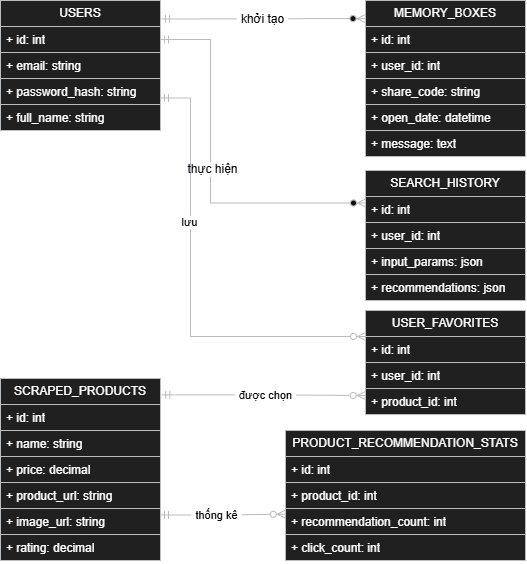
\includegraphics[width=0.92\textwidth]{chapters/diagram/ERD.drawio.png}
\caption{Lược đồ quan hệ thực thể (ERD) của hệ thống cơ sở dữ liệu GiftAI.}
\label{fig:erd_diagram}
\end{figure}

Lược đồ ERD trên minh họa mối quan hệ giữa 6 bảng dữ liệu trong CSDL phân tán TiDB Cloud. Bảng \texttt{USERS} đóng vai trò trung tâm với các mối quan hệ một-nhiều ($1:N$) tới \texttt{USER\_FAVORITES} (lưu các món quà đã thả tim), \texttt{SEARCH\_HISTORY} (lưu vết các phiên tư vấn) và \texttt{MEMORY\_BOXES} (quản lý các hộp quà đã tạo). Bảng \texttt{SEARCH\_HISTORY} tiếp tục liên kết một-nhiều tới \texttt{PRODUCT\_RECOMMENDATION\_STATS} nhằm theo dõi lượt hiển thị và số lần click của từng món quà trong phiên tìm kiếm đó. Bảng \texttt{SCRAPED\_PRODUCTS} hoạt động như một kho catalog trung tâm độc lập, liên tục cung cấp dữ liệu sản phẩm cho toàn bộ các quy trình tư vấn AI và gắn quà vào hộp kỷ niệm. Thiết kế chuẩn hóa 3NF này giúp triệt tiêu hiện tượng dư thừa dữ liệu và bảo đảm tính toàn vẹn thông tin trên môi trường Cloud.

% ---------------------------------------------------------------------
\section{Thiết kế thành phần tri thức và mô hình AI}

Thành phần AI không đóng vai trò một bộ phân lớp độc lập mà là một hạt nhân điều phối tri thức (\textit{Knowledge Orchestrator}):
\begin{itemize}[leftmargin=1.2cm, itemsep=2pt]
    \item \textbf{Cơ chế biểu diễn tri thức bằng Prompt Engineering:} Hệ thống chuyển hóa tri thức về tâm lý học xã hội, quy chuẩn tặng quà văn hóa Việt Nam (ngày 20/10 nên tặng hoa/mỹ phẩm, tân gia nên tặng đồ gia dụng) vào các câu lệnh hệ thống (\textit{System Prompt}).
    \item \textbf{Chiến lược gợi ý kết hợp (Hybrid Strategy):} Kết hợp giữa năng lực suy diễn không nhãn (\textit{Zero-shot}) của Google Gemini 3.8 Flash với kho hàng hóa $1.400+$ sản phẩm chuẩn hóa trên TiDB Cloud. Nhờ đó, hệ thống vừa nắm bắt được cảm xúc tinh tế, vừa cung cấp sản phẩm có thật 100\% trên thị trường.
\end{itemize}

% =====================================================================
% PHẦN II: ĐẶC TẢ CHI TIẾT VÀ LUỒNG CHỨC NĂNG (SRS CHI TIẾT)
% =====================================================================

\section{Mô hình hóa ca sử dụng (Use Case Modeling)}

\subsection{Biểu đồ ca sử dụng hệ thống}
Sơ đồ ca sử dụng của phân hệ Người dùng và Quản trị viên được thể hiện tại Hình~\ref{fig:user_uc} và Hình~\ref{fig:admin_uc}.

\begin{figure}[htbp]
\centering
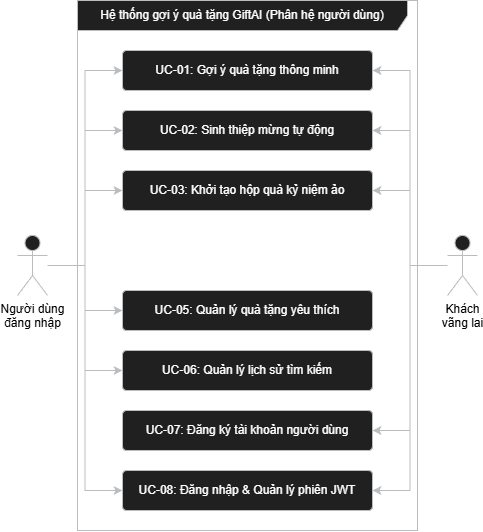
\includegraphics[width=0.88\textwidth]{chapters/diagram/UserUsecase.drawio.png}
\caption{Biểu đồ ca sử dụng phân hệ Người dùng (User Use Case Diagram).}
\label{fig:user_uc}
\end{figure}

Biểu đồ ca sử dụng phân hệ Người dùng mô tả sự tương tác của hai tác nhân là Khách vãng lai và Thành viên đã đăng nhập với 8 ca sử dụng thuộc phân hệ người dùng cuối. Người dùng có thể tiến hành khảo sát và nhận gợi ý quà tặng ngay lập tức mà không bắt buộc phải đăng nhập. Tuy nhiên, khi cần sử dụng các tính năng lưu trữ cá nhân như lưu quà yêu thích, xem lại lịch sử hoặc quản lý hộp quà của mình, hệ thống sẽ kích hoạt luồng xác thực tài khoản qua JWT.

\begin{figure}[htbp]
\centering
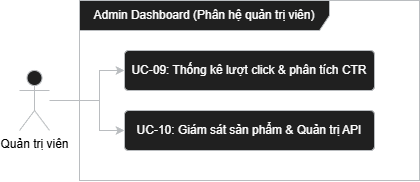
\includegraphics[width=0.88\textwidth]{chapters/diagram/AdminUsecase.drawio.png}
\caption{Biểu đồ ca sử dụng phân hệ Quản trị viên (Admin Use Case Diagram).}
\label{fig:admin_uc}
\end{figure}

Biểu đồ ca sử dụng phân hệ Quản trị viên thể hiện quyền hạn của tác nhân Admin trong việc kiểm soát toàn bộ hoạt động của hệ sinh thái GiftAI. Quản trị viên có quyền truy cập vào trang Admin Dashboard để theo dõi các biểu đồ thống kê lượt tương tác, tỷ lệ nhấp chuột CTR của từng danh mục sản phẩm, đồng thời giám sát trạng thái của các khóa API Gemini và tình trạng đồng bộ dữ liệu của kho hàng trên TiDB Cloud.

\subsection{Ma trận phân loại 10 ca sử dụng}

\begin{table}[htbp]
\centering
\caption{Ma trận phân loại 10 ca sử dụng trọng tâm của hệ thống GiftAI.}
\label{tab:uc_matrix}
\small
\renewcommand{\arraystretch}{1.25}
\begin{tabularx}{\textwidth}{|p{1.8cm}|p{5.5cm}|p{3.2cm}|X|}
\hline
\rowcolor{PrimaryBlue}
\textcolor{white}{\textbf{Mã UC}} &
\textcolor{white}{\textbf{Tên ca sử dụng}} &
\textcolor{white}{\textbf{Tác nhân chính}} &
\textcolor{white}{\textbf{Phân hệ chức năng}} \\
\hline
\textbf{UC-01} & Gợi ý quà tặng thông minh & Khách / Thành viên & Core AI Recommendation \\
\hline
\textbf{UC-02} & Sinh thiệp chúc mừng tự động & Khách / Thành viên & Generative Content \\
\hline
\textbf{UC-03} & Khởi tạo Hộp quà kỷ niệm ảo & Khách / Thành viên & Virtual Memory Box \\
\hline
\textbf{UC-04} & Mở khóa \& Xem Hộp quà kỷ niệm & Người nhận quà & Virtual Memory Box \\
\hline
\textbf{UC-05} & Quản lý quà tặng yêu thích & Thành viên đã đăng nhập & User Personalization \\
\hline
\textbf{UC-06} & Quản lý lịch sử tìm kiếm & Thành viên đã đăng nhập & User Personalization \\
\hline
\textbf{UC-07} & Đăng ký tài khoản người dùng & Khách vãng lai & Authentication \\
\hline
\textbf{UC-08} & Đăng nhập \& Quản lý phiên JWT & Khách / Thành viên & Authentication \\
\hline
\textbf{UC-09} & Thống kê lượt click \& Phân tích CTR & Quản trị viên & Analytics \& Tracking \\
\hline
\textbf{UC-10} & Giám sát sản phẩm \& Quản trị API & Quản trị viên & System Management \\
\hline
\end{tabularx}
\end{table}

Ma trận trên phân loại toàn diện 10 ca sử dụng trọng tâm của hệ thống thành 6 nhóm nghiệp vụ chính: Đề xuất quà tặng bằng AI, Sáng tạo nội dung thiệp, Hộp quà kỷ niệm, Cá nhân hóa người dùng, Xác thực phân quyền và Giám sát quản trị. Sự phân định này là cơ sở trực tiếp để xây dựng các kịch bản kiểm thử chức năng (Test Cases) được thực thi trong Chương V.

% ---------------------------------------------------------------------
\section{Đặc tả kỹ thuật chi tiết toàn bộ các ca sử dụng}

\subsection{UC-01: Gợi ý quà tặng thông minh (Intelligent Recommendation Engine)}

\begin{table}[htbp]
\centering
\caption{Bảng đặc tả kỹ thuật ca sử dụng UC-01.}
\label{tab:spec_uc01}
\small
\renewcommand{\arraystretch}{1.2}
\begin{tabularx}{\textwidth}{|p{3.2cm}|X|}
\hline
\rowcolor{PrimaryBlue}
\textcolor{white}{\textbf{Thuộc tính}} & \textcolor{white}{\textbf{Nội dung đặc tả chi tiết}} \\
\hline
\textbf{Mã định danh} & \textbf{UC-01: Intelligent Gift Recommendation Engine} \\
\hline
\textbf{Tác nhân} & Khách vãng lai, Thành viên, AI Manager, TiDB Cloud Database \\
\hline
\textbf{Mô tả} & Tiếp nhận thông tin hồ sơ người nhận đa tiêu chí và mô tả tự do; hệ thống phân rã ý định qua Gemini 3.8 Flash, truy xuất kho sản phẩm TiDB Cloud và thực hiện tái xếp hạng (Re-ranking) để đưa ra danh mục quà tặng tối ưu kèm lý giải thuyết phục. \\
\hline
\textbf{Tiền điều kiện} & Máy chủ Backend Render kết nối thành công với TiDB Cloud qua SSL; ít nhất một API Key còn hạn ngạch. \\
\hline
\textbf{Dữ liệu đầu vào} & Gói tin HTTP POST gửi tới \texttt{/api/recommend}: \texttt{relationship}, \texttt{gender}, \texttt{age}, \texttt{occasion}, \texttt{budget}, \texttt{interests}, \texttt{description}. \\
\hline
\textbf{Dữ liệu đầu ra} & Đối tượng JSON chứa: \texttt{success}, \texttt{ai} (\texttt{summary}, \texttt{items}, \texttt{keywords}) và mảng \texttt{products} (gồm: \texttt{name}, \texttt{price}, \texttt{image}, \texttt{url}, \texttt{platform}, \texttt{reason}, \texttt{score}). \\
\hline
\textbf{Hậu điều kiện} & Ghi nhận lượt tìm kiếm vào bảng \texttt{search\_history}; tăng số lượt hiển thị tương ứng trong bảng \texttt{product\_recommendation\_stats}; lưu kết quả vào RAM Cache. \\
\hline
\end{tabularx}
\end{table}

Quy trình thực thi của ca sử dụng UC-01 diễn ra qua các bước tuần tự: Người dùng nhập thông tin khảo sát trên giao diện Web hoặc Android và bấm tìm quà. Backend tiếp nhận gói tin, tính toán mã băm của dữ liệu đầu vào để kiểm tra trong bộ đệm RAM Cache. Nếu có sẵn trong bộ đệm (Cache Hit), kết quả được phản hồi ngay lập tức trong vòng dưới $10\text{ ms}$. Nếu trượt bộ đệm (Cache Miss), Backend kích hoạt mô hình Gemini 3.8 Flash để trích xuất ý định và sinh từ khóa. Tiếp theo, hệ thống truy vấn kho $1.400+$ sản phẩm trên TiDB Cloud; nếu thiếu hàng, worker Selenium sẽ cào bổ sung từ Shopee/Lazada. Tập ứng viên sản phẩm sau đó được đưa vào Prompt tái xếp hạng của Gemini 3.8 Flash để loại bỏ đồ rác, chấm điểm độ phù hợp và sinh lời giải thích tâm lý cho từng món đồ trước khi trả về cho Client.

% ---------------------------------------------------------
\subsection{UC-02: Sinh thiệp chúc mừng tự động (AI Greeting Card Generator)}

\begin{table}[htbp]
\centering
\caption{Bảng đặc tả kỹ thuật ca sử dụng UC-02.}
\label{tab:spec_uc02}
\small
\renewcommand{\arraystretch}{1.2}
\begin{tabularx}{\textwidth}{|p{3.2cm}|X|}
\hline
\rowcolor{PrimaryBlue}
\textcolor{white}{\textbf{Thuộc tính}} & \textcolor{white}{\textbf{Nội dung đặc tả chi tiết}} \\
\hline
\textbf{Mã định danh} & \textbf{UC-02: AI Greeting Card Generator} \\
\hline
\textbf{Tác nhân} & Khách vãng lai, Thành viên, AI Manager \\
\hline
\textbf{Mô tả} & Cho phép người dùng chọn một món quà cụ thể, lựa chọn phong cách biểu cảm mong muốn để AI tự động sáng tác thông điệp chúc mừng giàu cảm xúc, hiển thị trên thiệp mừng tương tác. \\
\hline
\textbf{Dữ liệu đầu vào} & Tên món quà (\texttt{productName}), Tên người nhận (\texttt{recipientName}), Dịp tặng (\texttt{occasion}), Tông giọng (\texttt{tone}: Hài hước, Chân thành, Lãng mạn, Trang trọng, Thơ ca), Mẫu thiệp đã chọn (\texttt{themeId}). \\
\hline
\textbf{Dữ liệu đầu ra} & Văn bản lời chúc mừng do AI sinh ra, xem trước thiệp mừng theo thời gian thực kèm hiệu ứng pháo hoa mở hộp quà. \\
\hline
\end{tabularx}
\end{table}

Ca sử dụng UC-02 cho phép người dùng biến một món quà vô tri thành một thông điệp tình cảm tinh tế. Người dùng chọn món quà và bấm nút "Tạo thiệp chúc mừng", chọn tông giọng phù hợp như lãng mạn, hài hước hay thơ lục bát. Mô hình AI dựa trên các thông số này để sinh ra đoạn văn hoặc bài thơ 4 câu đầy cảm xúc trong vòng 1.5 giây. Người dùng có thể chỉnh sửa lại từ ngữ trực tiếp trên giao diện thiệp 3D, đổi mẫu nền và lưu lại để đính kèm vào Hộp kỷ niệm ảo hoặc gửi trực tiếp cho người nhận.

% ---------------------------------------------------------
\subsection{UC-03: Khởi tạo Hộp quà kỷ niệm ảo (Virtual Memory Box Creation)}

\begin{table}[htbp]
\centering
\caption{Bảng đặc tả kỹ thuật ca sử dụng UC-03.}
\label{tab:spec_uc03}
\small
\renewcommand{\arraystretch}{1.2}
\begin{tabularx}{\textwidth}{|p{3.2cm}|X|}
\hline
\rowcolor{PrimaryBlue}
\textcolor{white}{\textbf{Thuộc tính}} & \textcolor{white}{\textbf{Nội dung đặc tả chi tiết}} \\
\hline
\textbf{Mã định danh} & \textbf{UC-03: Virtual Memory Box Creation} \\
\hline
\textbf{Tác nhân} & Người tặng quà (Khách hoặc Thành viên), Backend API, TiDB Cloud Database \\
\hline
\textbf{Mô tả} & Người tặng đóng gói món quà vật lý, bức tâm thư và thiệp chúc mừng vào chiếc hộp số; thiết lập ngày kỷ niệm đếm ngược và nhận mã chia sẻ độc nhất \texttt{share\_code} để gửi cho người nhận. \\
\hline
\textbf{Dữ liệu đầu vào} & Tiêu đề hộp quà (\texttt{title}), Tên người gửi/người nhận, Dịp lễ (\texttt{occasion}), Kiểu đếm (\texttt{milestone\_type}), Mốc ngày (\texttt{milestone\_date}), Lời tâm thư (\texttt{letter\_content}), Món quà đính kèm. \\
\hline
\textbf{Dữ liệu đầu ra} & Mã định danh chia sẻ duy nhất (\texttt{share\_code}) dạng \texttt{MEM-XXXXXX} và liên kết URL công khai. \\
\hline
\textbf{Hậu điều kiện} & Tạo một bản ghi mới trong bảng \texttt{memory\_boxes} trên TiDB Cloud với \texttt{unboxed\_count = 0}. \\
\hline
\end{tabularx}
\end{table}

Trong ca sử dụng UC-03, người tặng quà khởi tạo một không gian kỷ niệm số dành riêng cho người nhận. Sau khi nhập các thông điệp tâm thư, thiết lập ngày bắt đầu yêu nhau hoặc ngày đếm ngược tới sinh nhật, hệ thống tự động sinh một chuỗi mã độc bản không trùng lặp có tiền tố \texttt{MEM-} bằng thư viện mã hóa bảo mật \texttt{crypto}. Bản ghi được lưu trữ an toàn trong bảng \texttt{memory\_boxes} trên TiDB Cloud và hệ thống cung cấp đường link chia sẻ dạng \texttt{https://giftfinder.vn/?box=MEM-XXXXXX} để người tặng gửi qua các ứng dụng nhắn tin.

% ---------------------------------------------------------
\subsection{UC-04: Mở khóa và Xem Hộp quà kỷ niệm (Memory Box Unlocking \& Viewing)}

\begin{table}[htbp]
\centering
\caption{Bảng đặc tả kỹ thuật ca sử dụng UC-04.}
\label{tab:spec_uc04}
\small
\renewcommand{\arraystretch}{1.2}
\begin{tabularx}{\textwidth}{|p{3.2cm}|X|}
\hline
\rowcolor{PrimaryBlue}
\textcolor{white}{\textbf{Thuộc tính}} & \textcolor{white}{\textbf{Nội dung đặc tả chi tiết}} \\
\hline
\textbf{Mã định danh} & \textbf{UC-04: Memory Box Unlocking and Viewing} \\
\hline
\textbf{Tác nhân} & Người nhận quà, Backend API, TiDB Cloud Database \\
\hline
\textbf{Mô tả} & Người nhận truy cập vào đường dẫn có mã \texttt{share\_code}, bấm mở hộp để kích hoạt hiệu ứng pháo hoa, xem thiệp chúc mừng, thông điệp tâm thư, đồng hồ đếm ngày và món quà đính kèm. \\
\hline
\textbf{Dữ liệu đầu vào} & Mã chia sẻ (\texttt{share\_code}) lấy từ URL tham số. \\
\hline
\textbf{Dữ liệu đầu ra} & Toàn bộ dữ liệu hộp quà được hiển thị: thiệp mừng, tâm thư, đồng hồ đếm ngày, hiệu ứng pháo hoa Confetti và món quà. \\
\hline
\textbf{Hậu điều kiện} & Cập nhật tăng biến đếm số lần mở hộp \texttt{unboxed\_count} lên 1 đơn vị trong bảng \texttt{memory\_boxes}. \\
\hline
\end{tabularx}
\end{table}

Ca sử dụng UC-04 tối ưu hóa sự thuận tiện cho người nhận quà. Khi mở liên kết chia sẻ trên điện thoại hoặc máy tính, người nhận thấy hình ảnh chiếc hộp quà được thắt nơ trang trọng. Chỉ với một cú nhấp chuột vào nút "Mở hộp quà", hiệu ứng nắp hộp mở ra kết hợp pháo hoa giấy bung nở, bản nhạc êm dịu phát lên và bức thiệp cùng món quà người tặng gửi gắm hiện ra trọn vẹn. Đồng thời, hệ thống tự động tăng trường \texttt{unboxed\_count} để ghi nhận lượt xem thành công.

% ---------------------------------------------------------
\subsection{UC-05: Quản lý Quà yêu thích (User Favorites Management)}

\begin{table}[htbp]
\centering
\caption{Bảng đặc tả kỹ thuật ca sử dụng UC-05.}
\label{tab:spec_uc05}
\small
\renewcommand{\arraystretch}{1.2}
\begin{tabularx}{\textwidth}{|p{3.2cm}|X|}
\hline
\rowcolor{PrimaryBlue}
\textcolor{white}{\textbf{Thuộc tính}} & \textcolor{white}{\textbf{Nội dung đặc tả chi tiết}} \\
\hline
\textbf{Mã định danh} & \textbf{UC-05: User Favorites Management} \\
\hline
\textbf{Tác nhân} & Thành viên đã đăng nhập, Backend API, TiDB Cloud Database \\
\hline
\textbf{Mô tả} & Cho phép người dùng bấm nút thả tim lưu lại các món quà ưng ý vào bảng \texttt{user\_favorites} cá nhân để xem lại sau hoặc xóa khỏi danh sách khi không còn nhu cầu. \\
\hline
\textbf{Tiền điều kiện} & Người dùng đã đăng nhập thành công và sở hữu mã JWT Token hợp lệ. \\
\hline
\textbf{Dữ liệu đầu vào} & Header: \texttt{Authorization: Bearer <token>}; Body: \texttt{product\_name}, \texttt{product\_price}, \texttt{product\_image}, \texttt{product\_url}, \texttt{platform}, \texttt{score}. \\
\hline
\textbf{Dữ liệu đầu ra} & JSON: \texttt{success: true}, thông báo trạng thái cập nhật và danh sách yêu thích mới nhất. \\
\hline
\end{tabularx}
\end{table}

Khi người dùng nhấn vào biểu tượng trái tim trên thẻ sản phẩm, ứng dụng kiểm tra mã JWT trong bộ nhớ trình duyệt. Nếu người dùng chưa đăng nhập, hộp thoại xác thực sẽ tự động xuất hiện. Nếu đã đăng nhập, yêu cầu \texttt{POST /api/user/favorites} được gửi đến Backend để thêm hoặc xóa sản phẩm khỏi bảng \texttt{user\_favorites} trên TiDB Cloud, biểu tượng trái tim chuyển sang màu đỏ rực rỡ báo hiệu món quà đã được lưu trữ thành công vào bộ sưu tập cá nhân.

% ---------------------------------------------------------
\subsection{UC-06: Quản lý Lịch sử tìm kiếm (Search History Management)}

\begin{table}[htbp]
\centering
\caption{Bảng đặc tả kỹ thuật ca sử dụng UC-06.}
\label{tab:spec_uc06}
\small
\renewcommand{\arraystretch}{1.2}
\begin{tabularx}{\textwidth}{|p{3.2cm}|X|}
\hline
\rowcolor{PrimaryBlue}
\textcolor{white}{\textbf{Thuộc tính}} & \textcolor{white}{\textbf{Nội dung đặc tả chi tiết}} \\
\hline
\textbf{Mã định danh} & \textbf{UC-06: Search History Management} \\
\hline
\textbf{Tác nhân} & Thành viên đã đăng nhập, Backend API, TiDB Cloud Database \\
\hline
\textbf{Mô tả} & Cho phép người dùng xem lại toàn bộ các lần tìm kiếm trước đây, xem lại các kết quả gợi ý AI đã đề xuất thông qua trường \texttt{products\_snapshot} mà không cần tốn thời gian nhập liệu lại từ đầu. \\
\hline
\textbf{Dữ liệu đầu vào} & Header: \texttt{Authorization: Bearer <token>}; Phương thức \texttt{GET /api/user/history}. \\
\hline
\textbf{Dữ liệu đầu ra} & Mảng danh sách các phiên tìm kiếm gồm: thời gian tìm kiếm, mối quan hệ, dịp tặng, ngân sách, phân tích AI và danh sách sản phẩm snapshot. \\
\hline
\end{tabularx}
\end{table}

Mỗi lượt tìm kiếm thành công của thành viên đều được ghi nhận vào bảng \texttt{search\_history}. Khi người dùng truy cập màn hình "Lịch sử tìm kiếm", ứng dụng nạp danh sách các phiên tư vấn trong quá khứ sắp xếp theo thời gian mới nhất. Nhờ việc đọc trực tiếp dữ liệu từ cột \texttt{products\_snapshot}, giao diện hiển thị ngay tức thì danh sách sản phẩm cùng mức giá tại thời điểm tìm kiếm mà không cần gọi lại mô hình AI, giúp người dùng dễ dàng xem lại các phương án quà tặng đã được gợi ý trước đó.

% ---------------------------------------------------------
\subsection{UC-07 \& UC-08: Đăng ký, Đăng nhập và Xác thực phiên JWT}

\begin{table}[htbp]
\centering
\caption{Bảng đặc tả kỹ thuật ca sử dụng Xác thực người dùng (UC-07 \& UC-08).}
\label{tab:spec_uc_auth}
\small
\renewcommand{\arraystretch}{1.2}
\begin{tabularx}{\textwidth}{|p{3.2cm}|X|}
\hline
\rowcolor{PrimaryBlue}
\textcolor{white}{\textbf{Thuộc tính}} & \textcolor{white}{\textbf{Nội dung đặc tả chi tiết}} \\
\hline
\textbf{Mã định danh} & \textbf{UC-07: Registration \& UC-08: Login and JWT Authentication} \\
\hline
\textbf{Tác nhân} & Khách vãng lai, Thành viên, Middleware Auth, TiDB Cloud Database \\
\hline
\textbf{Mô tả} & Đăng ký tài khoản mới bằng Email và Mật khẩu; Đăng nhập hệ thống, kiểm tra tính toàn vẹn mật khẩu và cấp phát mã JSON Web Token (JWT) để bảo vệ các tuyến API nhạy cảm. \\
\hline
\textbf{Quy tắc nghiệp vụ} & Mật khẩu được băm một chiều an toàn bằng thuật toán \texttt{bcrypt} (10 salt rounds); Token JWT ký bằng khóa bí mật máy chủ và có thời hạn sống 7 ngày. \\
\hline
\textbf{Dữ liệu đầu vào} & \texttt{email} (đúng định dạng email chuẩn), \texttt{password} (độ dài tối thiểu 6 ký tự), \texttt{full\_name}. \\
\hline
\textbf{Dữ liệu đầu ra} & Đối tượng người dùng (\texttt{id}, \texttt{email}, \texttt{role}, \texttt{full\_name}) và chuỗi mã \texttt{token}. \\
\hline
\end{tabularx}
\end{table}

Quy trình xác thực diễn ra thông qua hai endpoint \texttt{/api/auth/register} và \texttt{/api/auth/login}. Khi đăng ký, máy chủ kiểm tra tính duy nhất của email trên bảng \texttt{users}, băm mật khẩu qua thư viện \texttt{bcryptjs} rồi lưu trữ bản ghi mới. Khi đăng nhập, hàm so sánh \texttt{bcrypt.compare()} đối chiếu mật khẩu nhập vào với mã băm trong CSDL. Nếu khớp, máy chủ cấp phát mã JWT ký bằng thuật toán HMAC-SHA256 có thời hạn 7 ngày. Trình duyệt lưu mã này vào \texttt{localStorage} và tự động đính kèm vào tiêu đề \texttt{Authorization: Bearer <token>} trong mọi yêu cầu cần xác thực quyền truy cập.

% ---------------------------------------------------------
\subsection{UC-09: Thống kê lượt click \& Phân tích tỷ lệ CTR (Analytics \& Tracking)}

\begin{table}[htbp]
\centering
\caption{Bảng đặc tả kỹ thuật ca sử dụng UC-09.}
\label{tab:spec_uc09}
\small
\renewcommand{\arraystretch}{1.2}
\begin{tabularx}{\textwidth}{|p{3.2cm}|X|}
\hline
\rowcolor{PrimaryBlue}
\textcolor{white}{\textbf{Thuộc tính}} & \textcolor{white}{\textbf{Nội dung đặc tả chi tiết}} \\
\hline
\textbf{Mã định danh} & \textbf{UC-09: Click Tracking \& CTR Analytics} \\
\hline
\textbf{Tác nhân} & Người dùng (khi click xem/mua quà), Quản trị viên, Backend API \\
\hline
\textbf{Mô tả} & Ghi nhận hành vi người dùng khi nhấp vào nút xem/mua trên từng sản phẩm, tự động cập nhật số lượt click (\texttt{clicks}) trong bảng \texttt{product\_recommendation\_stats} để phục vụ quản trị phân tích xu hướng. \\
\hline
\textbf{Công thức đo lường} & Tỷ lệ nhấp chuột được hệ thống tính tự động:
$\mathrm{CTR} = \frac{\sum \mathrm{Clicks}}{\sum \mathrm{Impressions}} \times 100\%$. \\
\hline
\textbf{Hậu điều kiện} & Cập nhật bản ghi trong bảng \texttt{product\_recommendation\_stats}; hiển thị biểu đồ trên giao diện Admin Dashboard. \\
\hline
\end{tabularx}
\end{table}

Mỗi khi người dùng nhấp vào nút chuyển hướng sang gian hàng Shopee hoặc Lazada trên một thẻ quà tặng, hệ thống ngầm gửi yêu cầu tới API đo lường nhằm tăng biến đếm số lượt nhấp chuột \texttt{clicks} trong bảng \texttt{product\_recommendation\_stats}. Tại giao diện Admin Dashboard, số liệu này được tổng hợp cùng số lượt hiển thị \texttt{impressions} để vẽ biểu đồ phân tích tỷ lệ CTR theo từng danh mục hàng hóa, giúp người quản trị dễ dàng nhận diện những xu hướng quà tặng đang được người dùng quan tâm nhiều nhất.

% ---------------------------------------------------------
\subsection{UC-10: Giám sát sản phẩm \& Quản trị API (System Management)}

\begin{table}[htbp]
\centering
\caption{Bảng đặc tả kỹ thuật ca sử dụng UC-10.}
\label{tab:spec_uc10}
\small
\renewcommand{\arraystretch}{1.2}
\begin{tabularx}{\textwidth}{|p{3.2cm}|X|}
\hline
\rowcolor{PrimaryBlue}
\textcolor{white}{\textbf{Thuộc tính}} & \textcolor{white}{\textbf{Nội dung đặc tả chi tiết}} \\
\hline
\textbf{Mã định danh} & \textbf{UC-10: Product Monitoring \& API Administration} \\
\hline
\textbf{Tác nhân} & Quản trị viên hệ thống (Admin) \\
\hline
\textbf{Mô tả} & Giám sát các tham số vận hành: số lượng $1.400+$ sản phẩm trong kho CSDL TiDB Cloud, tình trạng kết nối tới các sàn TMĐT, danh sách các khóa API Gemini còn hoạt động và khóa bị vượt hạn mức (429). \\
\hline
\textbf{Tiền điều kiện} & Tài khoản đăng nhập phải có thuộc tính phân quyền \texttt{role = 'admin'}. \\
\hline
\end{tabularx}
\end{table}

Ca sử dụng UC-10 cung cấp giao diện quản trị chuyên sâu dành riêng cho tài khoản có quyền Admin. Hệ thống hiển thị bảng điều khiển trực quan về dung lượng và số lượng sản phẩm trong kho CSDL TiDB Cloud, trạng thái của 4 khóa API Google Gemini đang chạy luân phiên, số lượt lỗi HTTP 429 phát sinh trong ngày và nhật ký kích hoạt bộ chuyển mạch dự phòng Groq. Nhờ đó, người quản trị có thể chủ động bổ sung khóa API mới hoặc kích hoạt các đợt cào dữ liệu định kỳ để làm mới danh mục quà tặng.

% ---------------------------------------------------------------------
\section{Thiết kế luồng hoạt động chi tiết (Workflows \& State Transitions)}

\subsection{Biểu đồ tuần tự ca sử dụng Gợi ý quà tặng thông minh (Sequence Diagram)}
Sơ đồ tuần tự thể hiện các thông điệp trao đổi đồng bộ và bất đồng bộ giữa các đối tượng trong UC-01 được mô tả tại Hình~\ref{fig:seq_diagram}.

\begin{figure}[htbp]
\centering
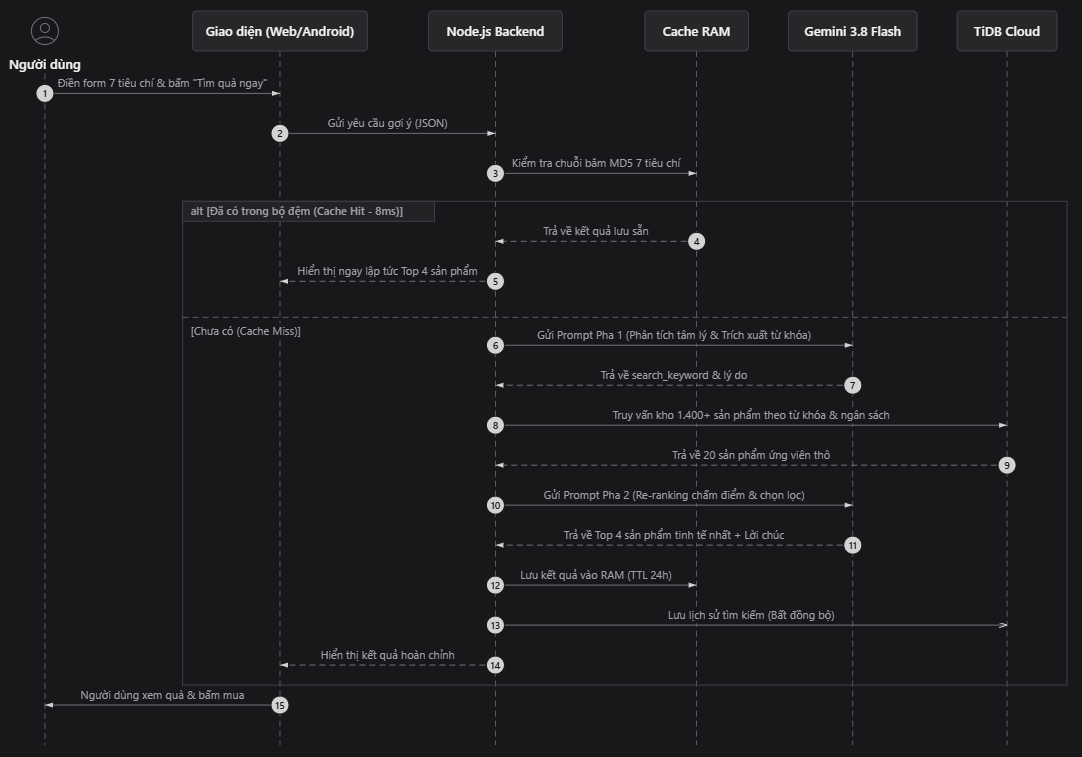
\includegraphics[width=0.95\textwidth]{chapters/diagram/sequence.drawio.png.png}
\caption{Biểu đồ tuần tự ca sử dụng Gợi ý quà tặng thông minh (Sequence Diagram).}
\label{fig:seq_diagram}
\end{figure}

Biểu đồ tuần tự trên mô tả chi tiết thứ tự truyền nhận thông điệp theo trục thời gian giữa 5 đối tượng: Người dùng (Client), Máy chủ Express Backend, Bộ đệm In-Memory Cache, CSDL TiDB Cloud và Mô hình Gemini 3.8 Flash. Sau khi tiếp nhận tiêu chí tìm kiếm, Backend kiểm tra bộ đệm RAM Cache. Nếu có sẵn trong bộ đệm, dữ liệu được trả về ngay trong $10\text{ ms}$. Nếu chưa có, Backend gọi Gemini 3.8 Flash trích xuất ý định, truy vấn kho $1.400+$ sản phẩm trên TiDB Cloud, đưa danh sách thô vào Prompt tái xếp hạng để lọc rác và sinh lý do tâm lý. Cuối cùng, kết quả được lưu vào RAM Cache, đồng thời việc ghi nhận lịch sử và đo lường click được thực thi bất đồng bộ ở chế độ nền để không làm tăng thời gian chờ đợi của người dùng.

\subsection{Biểu đồ tiến trình Tạo thiệp mừng và Khởi tạo Hộp quà kỷ niệm}
Tiến trình nghiệp vụ khi người dùng thiết kế thiệp chúc mừng tự động và đóng gói hộp quà số được thể hiện lần lượt tại Hình~\ref{fig:progress_card} và Hình~\ref{fig:progress_box}.

\begin{figure}[htbp]
\centering
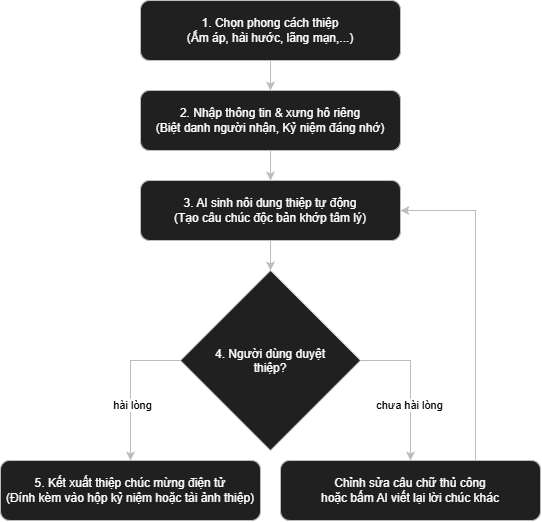
\includegraphics[width=0.65\textwidth]{chapters/diagram/Progress1.drawio.png}
\caption{Biểu đồ tiến trình tạo thiệp chúc mừng AI (Greeting Card Workflow).}
\label{fig:progress_card}
\end{figure}

Biểu đồ tiến trình trên thể hiện các bước nghiệp vụ từ lúc người dùng nhấp chọn tính năng tạo thiệp từ một món quà cụ thể, nhập tên người nhận và chọn tông giọng cảm xúc mong muốn. Yêu cầu được gửi tới máy chủ để kích hoạt AI sáng tác lời chúc trong khoảng 1.5 giây. Nếu người dùng hài lòng, thiệp được hiển thị trên giao diện 3D với hiệu ứng mở nắp hộp quà; nếu chưa ưng ý, người dùng có thể bấm nút yêu cầu AI viết lại một lời chúc khác hoặc tự chỉnh sửa câu chữ theo ý muốn trước khi lưu trữ hoặc tải về.

\begin{figure}[htbp]
\centering
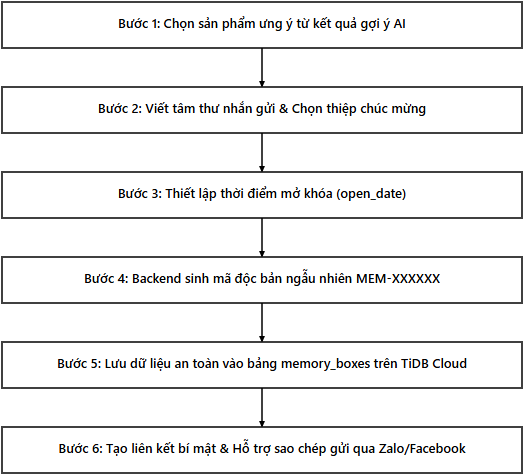
\includegraphics[width=0.65\textwidth]{chapters/diagram/Progress2.drawio.png}
\caption{Biểu đồ tiến trình khởi tạo Hộp quà kỷ niệm ảo (Memory Box Creation Workflow).}
\label{fig:progress_box}
\end{figure}

Tiến trình khởi tạo Hộp quà kỷ niệm ảo diễn ra qua các bước lựa chọn món quà vật lý, soạn thảo bức tâm thư, chọn phong cách thiệp nền và thiết lập ngày kỷ niệm đếm xuôi hay đếm ngược. Sau khi dữ liệu được kiểm tra hợp lệ, Backend sinh mã băm độc bản \texttt{share\_code} với tiền tố \texttt{MEM-}, lưu toàn bộ cấu trúc dữ liệu vào bảng \texttt{memory\_boxes} trên TiDB Cloud và xuất ra đường dẫn liên kết công khai để người gửi có thể sao chép và gửi ngay cho người nhận.

\subsection{Biểu đồ chuyển trạng thái Hộp quà kỷ niệm (State Machine Diagram)}
Vòng đời của Hộp quà kỷ niệm ảo trải qua các trạng thái chuyển dịch từ lúc khởi tạo đến khi người nhận mở hộp thành công, như mô tả tại Hình~\ref{fig:state_diagram}.

\begin{figure}[htbp]
\centering
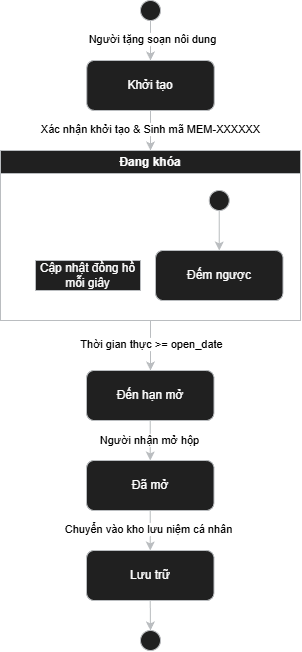
\includegraphics[width=0.4\textwidth]{chapters/diagram/StateDiagram.drawio.png}
\caption{Biểu đồ chuyển trạng thái Hộp quà kỷ niệm ảo (State Diagram).}
\label{fig:state_diagram}
\end{figure}

Biểu đồ máy trạng thái trên mô tả vòng đời hoàn chỉnh của một hộp quà kỷ niệm ảo trong hệ thống. Hộp quà bắt đầu ở trạng thái Khởi tạo (\textit{Draft}) khi người dùng đang soạn thảo. Khi người dùng bấm hoàn tất, hộp quà chuyển sang trạng thái Đã niêm phong (\textit{Sealed}) và mã \texttt{share\_code} được tạo ra để chuyển sang trạng thái Đang chia sẻ (\textit{Shared}). Khi người nhận nhấp vào liên kết và bấm nút mở nắp hộp, trạng thái chuyển sang Đã mở quà (\textit{Unboxed}), kích hoạt hiệu ứng pháo hoa, phát nhạc và tăng biến đếm số lượt mở hộp trong cơ sở dữ liệu.

\section{Tóm tắt chương}
Chương III đã hoàn thiện toàn diện bản phân tích và thiết kế kiến trúc hệ sinh thái GiftAI trên môi trường Cloud phân tán. Việc thiết kế mô hình dữ liệu chuẩn hóa 6 bảng trên TiDB Cloud Singapore kết hợp cơ chế Connection Pooling qua giao thức mã hóa SSL/TLSv1.2 đã giải quyết triệt để bài toán lưu trữ phân tán với độ trễ truy xuất dưới $15\text{ ms}$. Hệ thống 10 ca sử dụng cùng các biểu đồ luồng hoạt động UML chuẩn mực là nền tảng vững chắc để triển khai các giải pháp trí tuệ nhân tạo chuyên sâu được trình bày chi tiết trong Chương IV.